\documentclass[12pt,a4paper]{article}
\usepackage[utf8]{inputenc}
\usepackage[T1]{fontenc}
\usepackage{geometry}
\usepackage{amsmath}
\usepackage{amssymb}
\usepackage{booktabs}
\usepackage{hyperref}
\usepackage{parskip}
\usepackage{titlesec}
\usepackage{enumitem}
\usepackage{xcolor}
\usepackage{tcolorbox}
\usepackage{fancyhdr}
\usepackage{lmodern}
\usepackage{anyfontsize}
\usepackage{tikz}
\usepackage{fontawesome5}
\usepackage{mdframed}
\usepackage{colortbl}
\usepackage{tabularx}
\usepackage{graphicx}
\usepackage{float}

% Load tcolorbox libraries
\tcbuselibrary{skins,breakable}

% ========================
% COLOR PALETTE
% ========================
\definecolor{deepblue}{RGB}{41, 65, 122}
\definecolor{accentblue}{RGB}{52, 152, 219}
\definecolor{lightblue}{RGB}{214, 234, 248}
\definecolor{accentteal}{RGB}{26, 188, 156}
\definecolor{lightteal}{RGB}{212, 248, 239}
\definecolor{accentorange}{RGB}{243, 156, 18}
\definecolor{lightorange}{RGB}{253, 235, 208}
\definecolor{accentpurple}{RGB}{142, 68, 173}
\definecolor{lightpurple}{RGB}{235, 222, 240}
\definecolor{accentred}{RGB}{231, 76, 60}
\definecolor{lightred}{RGB}{250, 219, 216}
\definecolor{accentgreen}{RGB}{39, 174, 96}
\definecolor{lightgreen}{RGB}{212, 239, 223}
\definecolor{darkgray}{RGB}{44, 62, 80}
\definecolor{medgray}{RGB}{127, 140, 141}
\definecolor{tablegray}{RGB}{245, 247, 250}
\definecolor{tableheader}{RGB}{41, 65, 122}

\geometry{margin=2.5cm}

% ========================
% HYPERLINK SETUP
% ========================
\hypersetup{
    colorlinks=true,
    linkcolor=accentblue,
    urlcolor=accentteal,
    citecolor=accentpurple
}

% ========================
% PAGE STYLE
% ========================
\pagestyle{fancy}
\setlength{\headheight}{25pt}
\addtolength{\topmargin}{-13pt}
\fancyhf{}
\fancyhead[L]{\small\color{medgray}\textit{CMPE 49G -- Homework 2}}
\fancyhead[R]{\small\color{medgray}\textit{Particle Image Velocimetry}}
\fancyfoot[C]{\color{deepblue}\thepage}
\renewcommand{\headrulewidth}{0.4pt}
\renewcommand{\headrule}{\hbox to\headwidth{\color{accentblue}\leaders\hrule height \headrulewidth\hfill}}
\renewcommand{\footrulewidth}{0pt}

% ========================
% SECTION FORMATTING
% ========================
\titleformat{\section}
  {\normalfont\Large\bfseries\color{deepblue}}
  {\colorbox{deepblue}{\color{white}\,\thesection\,}}{0.8em}{}

\titleformat{\subsection}
  {\normalfont\large\bfseries\color{accentblue}}
  {\color{accentblue}\thesubsection}{0.6em}{}

\titleformat{\subsubsection}
  {\normalfont\normalsize\bfseries\color{accentpurple}}
  {\thesubsubsection}{0.5em}{}

% ========================
% CUSTOM TCOLORBOXES
% ========================

% Student Question Box
\newtcolorbox{questionbox}[1][]{%
    enhanced,
    breakable,
    colback=lightblue,
    colframe=accentblue,
    coltitle=white,
    fonttitle=\bfseries,
    title={\faIcon{user-graduate}~Student Question},
    left=8pt, right=8pt, top=6pt, bottom=6pt,
    boxrule=0pt,
    borderline west={3pt}{0pt}{accentblue},
    arc=2pt,
    #1
}

% LLM Answer Box
\newtcolorbox{answerbox}[1][]{%
    enhanced,
    breakable,
    colback=lightteal!30!white,
    colframe=accentteal,
    coltitle=white,
    fonttitle=\bfseries,
    title={\faIcon{robot}~LLM Answer},
    left=8pt, right=8pt, top=6pt, bottom=6pt,
    boxrule=0pt,
    borderline west={3pt}{0pt}{accentteal},
    arc=2pt,
    #1
}

% Important Concept Box
\newtcolorbox{conceptbox}[2][]{%
    enhanced,
    breakable,
    colback=lightpurple!40!white,
    colframe=accentpurple,
    coltitle=white,
    fonttitle=\bfseries,
    title={\faIcon{lightbulb}~#2},
    left=8pt, right=8pt, top=6pt, bottom=6pt,
    boxrule=0.8pt,
    arc=3pt,
    #1
}

% Warning/Limitation Box
\newtcolorbox{warningbox}[2][]{%
    enhanced,
    breakable,
    colback=lightorange!40!white,
    colframe=accentorange,
    coltitle=white,
    fonttitle=\bfseries,
    title={\faIcon{exclamation-triangle}~#2},
    left=8pt, right=8pt, top=6pt, bottom=6pt,
    boxrule=0.8pt,
    arc=3pt,
    #1
}

% Summary Box
\newtcolorbox{summarybox}[2][]{%
    enhanced,
    breakable,
    colback=lightgreen!40!white,
    colframe=accentgreen,
    coltitle=white,
    fonttitle=\bfseries,
    title={\faIcon{check-circle}~#2},
    left=8pt, right=8pt, top=6pt, bottom=6pt,
    boxrule=0.8pt,
    arc=3pt,
    #1
}

% Math highlight box
\newtcolorbox{mathbox}{%
    enhanced,
    colback=lightblue!25!white,
    colframe=accentblue!50!white,
    boxrule=0.5pt,
    arc=3pt,
    left=10pt, right=10pt, top=8pt, bottom=8pt
}

% ========================
% TABLE STYLING
% ========================
\newcommand{\tablemark}{\cellcolor{tableheader}\color{white}\bfseries}

% ========================
% TITLE PAGE
% ========================
\title{}
\author{}
\date{}

\begin{document}

% Custom Title Page
\begin{titlepage}
\begin{tikzpicture}[remember picture, overlay]
    % Background gradient blocks
    \fill[deepblue] (current page.north west) rectangle ([yshift=-8cm]current page.north east);
    \fill[accentblue!80!deepblue] ([yshift=-8cm]current page.north west) rectangle ([yshift=-8.3cm]current page.north east);
    \fill[accentteal!60!white] ([yshift=-8.3cm]current page.north west) rectangle ([yshift=-8.5cm]current page.north east);

    % Decorative circles
    \fill[accentblue, opacity=0.3] (14, -3) circle (3cm);
    \fill[accentteal, opacity=0.2] (15.5, -5) circle (2cm);
    \fill[accentpurple, opacity=0.15] (2, -6) circle (1.5cm);
    
    % Title text
    \node[anchor=west, text width=14cm] at (1.5, -2.5) {
        {\fontsize{14}{16}\selectfont\color{accentteal!70!white}\textbf{CMPE 49G -- Fundamentals of Particle-based Simulations}}
    };
    \node[anchor=west, text width=14cm] at (1.5, -4.5) {
        {\fontsize{26}{30}\selectfont\color{white}\textbf{Homework 2}}
    };
    \node[anchor=west, text width=14cm] at (1.5, -6) {
        {\fontsize{16}{18}\selectfont\color{cyan}\textit{Chat with LLM on Particle Image Velocimetry (PIV)}}
    };
    
    % Bottom info
    \node[anchor=west] at (1.5, -9.5) {
        {\large\color{blue}\faIcon{user-graduate}\quad\textbf{Student:} Ali Ayhan Günder - 2021400219}
    };
    \node[anchor=west] at (1.5, -10.5) {
        {\large\color{red}\faIcon{robot}\quad\textbf{LLM Used:} \textit{Claude Sonnet 4.6}}
    };
    \node[anchor=west] at (1.5, -11.5) {
        {\large\color{green}\faIcon{calendar-alt}\quad\textbf{Date:} March 14, 2026}
    };
    
    % Bottom decorative bar
    \fill[accentblue] (current page.south west) rectangle ([yshift=0.5cm]current page.south east);
    \fill[accentteal] ([yshift=0.5cm]current page.south west) rectangle ([yshift=0.7cm]current page.south east);
\end{tikzpicture}
\end{titlepage}

% ========================
% TABLE OF CONTENTS
% ========================
{
\hypersetup{linkcolor=deepblue}
\tableofcontents
}
\newpage

% ==============================================================
\section{AI Transparency Note}
% ==============================================================

\begin{tcolorbox}[
    enhanced,
    colback=lightblue!20!white,
    colframe=accentblue,
    boxrule=0.8pt,
    arc=4pt,
    left=12pt, right=12pt, top=10pt, bottom=10pt
]
\faIcon{info-circle}\;\textbf{Disclosure:} This report documents a structured chat session with \textbf{\color{accentblue}Claude Sonnet 4.6} on the topic of Particle Image Velocimetry (PIV). The questions were formulated by the student following the homework outline. The usage level is \textbf{\color{accentred}heavy}: the LLM was the primary source of information, and answers were reviewed and verified against standard PIV literature (Raffel et al., \textit{Particle Image Velocimetry: A Practical Guide}, 3rd~ed.). The student takes full responsibility for the submitted content.
\end{tcolorbox}

% ==============================================================
\section{Chat Log}
% ==============================================================

% --------------------------------------------------------------
\subsection{Q1: What is PIV? What is it used for in real life?}
% --------------------------------------------------------------

\begin{questionbox}
What is Particle Image Velocimetry (PIV)? What is it used for in real life?
\end{questionbox}

\begin{answerbox}
Particle Image Velocimetry (PIV) is an \textbf{\color{accentblue}optical, non-intrusive flow measurement technique} used to measure the velocity field of a fluid (liquid or gas) over a 2D plane---or a 3D volume in stereoscopic/tomographic variants---at an instant in time.

\begin{conceptbox}{How It Works Conceptually}
Small tracer particles chosen to closely follow the fluid motion (\emph{neutrally buoyant}) are seeded into the flow. A laser sheet illuminates a thin plane of the flow at two closely spaced instants, $t$ and $t + \Delta t$. A camera captures two frames. By statistically comparing how particle groups have moved between the two frames, the local velocity vector field is computed across the entire measurement plane.
\end{conceptbox}

\vspace{0.5em}
\textbf{\color{deepblue}\faIcon{globe}~Real-life Applications:}

\vspace{0.3em}
\begin{center}
\renewcommand{\arraystretch}{1.4}
\begin{tabularx}{\linewidth}{>{\bfseries\color{deepblue}}l X}
\toprule
\tablemark Domain & \tablemark Example \\
\midrule
\rowcolor{tablegray}
Aerospace & Wind tunnel studies of airfoil wakes, turbulent boundary layers \\
Automotive & Flow around vehicles, engine combustion studies \\
\rowcolor{tablegray}
Biomedical & Blood flow in arteries (micro-PIV), heart valve hemodynamics \\
Civil/Environmental & River flow, coastal wave dynamics \\
\rowcolor{tablegray}
Turbomachinery & Pump and turbine internal flows \\
Fundamental Research & Turbulence, vortex dynamics, mixing layers \\
\bottomrule
\end{tabularx}
\end{center}

\vspace{0.3em}
The key advantage over intrusive probes (hot-wire anemometry, Pitot tubes) is that PIV captures the \textbf{\color{accentgreen}whole-field velocity} simultaneously without disturbing the flow.

\begin{figure}[H]
    \centering
    \begin{tcolorbox}[
        enhanced,
        colback=lightblue!10!white,
        colframe=accentblue,
        boxrule=0.8pt,
        arc=4pt,
        left=6pt, right=6pt, top=6pt, bottom=4pt,
        title={\faIcon{wind}~PIV Velocity Field},
        coltitle=white,
        fonttitle=\bfseries\small
    ]
    \centering
    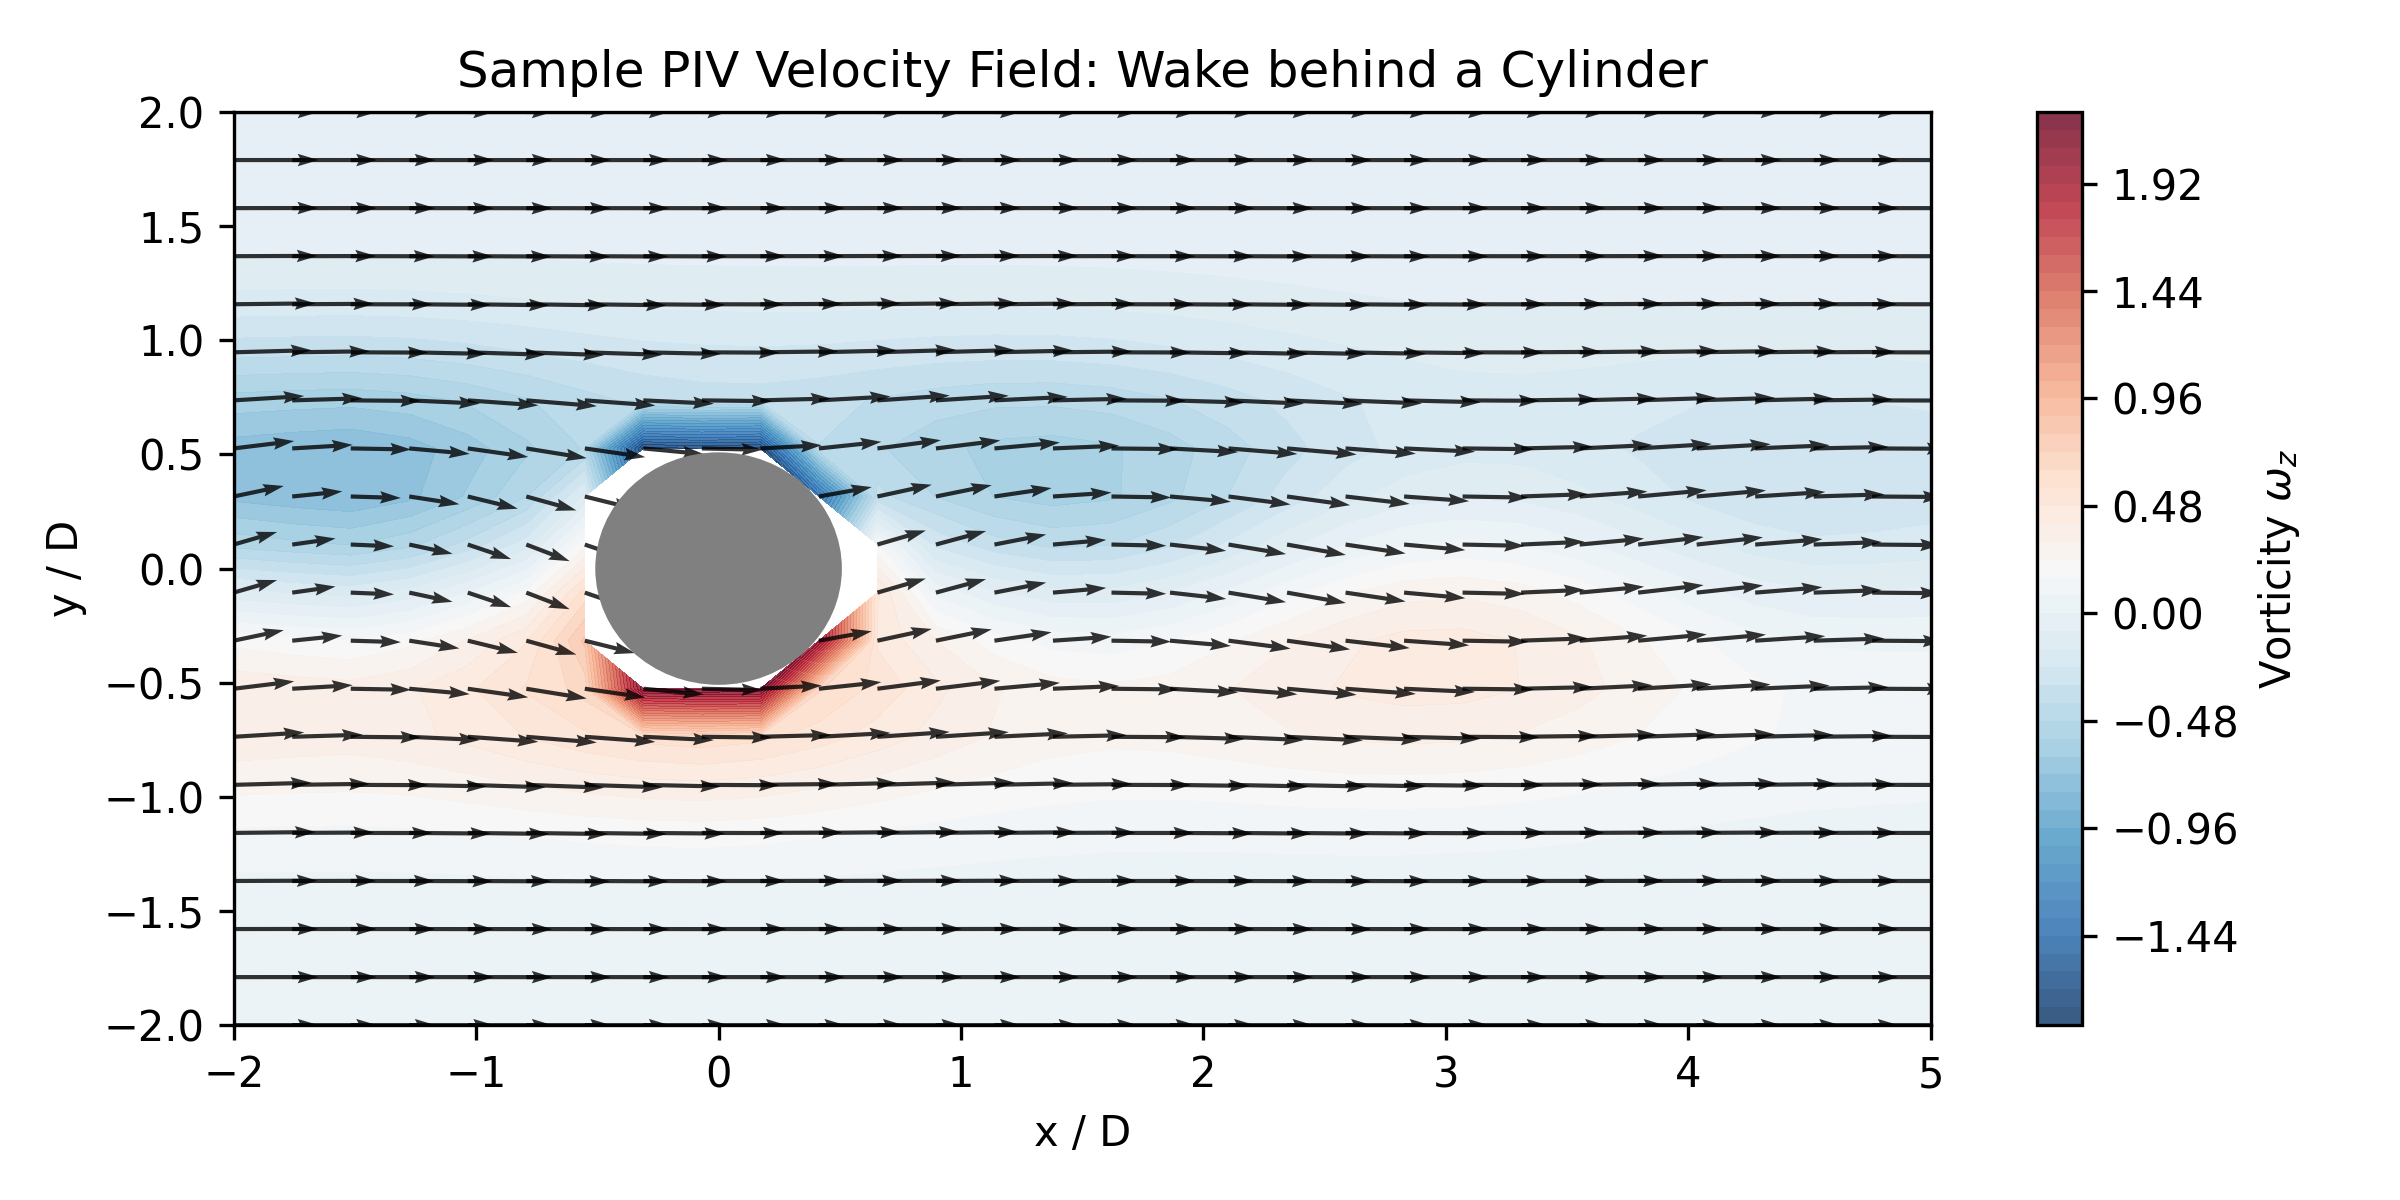
\includegraphics[width=\linewidth]{piv_velocity_field.png}
    \end{tcolorbox}
    \caption{Sample PIV velocity vector field overlaid on vorticity contours (simulated wake behind a cylinder).}
    \label{fig:piv_velocity}
\end{figure}
\end{answerbox}

% --------------------------------------------------------------
\subsection{Q2: What does ``non-intrusive'' mean?}
% --------------------------------------------------------------

\begin{questionbox}
You mentioned PIV is ``non-intrusive.'' What does that exactly mean?
\end{questionbox}

\begin{answerbox}
``Non-intrusive'' means the measurement technique does not physically insert any sensor or probe into the fluid. A Pitot tube or hot-wire anemometer must be placed inside the flow, which:
\begin{itemize}[noitemsep, leftmargin=1.5em]
    \item[\color{accentred}\faIcon{times-circle}] disturbs the flow field around the probe,
    \item[\color{accentred}\faIcon{times-circle}] measures only at a single point,
    \item[\color{accentred}\faIcon{times-circle}] can be impractical in hostile environments (high-temperature combustion, biological tissues).
\end{itemize}
PIV uses \textbf{\color{accentblue}light} (laser) to illuminate and a \textbf{\color{accentblue}camera} to observe---both from outside the flow domain. The only things inside the fluid are tracer particles, which are small enough (typically 1--100\,\textmu m) that they faithfully follow fluid streamlines without altering the flow behavior.
\end{answerbox}

% --------------------------------------------------------------
\subsection{Q3: What are the main physical components of a PIV system?}
% --------------------------------------------------------------

\begin{questionbox}
What are the main physical components required for a PIV system?
\end{questionbox}

\begin{answerbox}

\textbf{\color{deepblue}\faIcon{atom}~1. Tracer Particles (Seeding)}

Small particles that \textbf{follow the flow} (low Stokes number, $St \ll 1$). Common choices: hollow glass spheres (liquids), oil droplets, titanium dioxide ($\mathrm{TiO_2}$) powder (gas flows), polystyrene microspheres (micro-PIV). Particle diameter typically 1--100\,\textmu m.

\begin{mathbox}
The Stokes number is defined as:
\begin{equation}
    St = \frac{\tau_p}{\tau_f}
\end{equation}
where $\tau_p$ is the particle response time and $\tau_f$ is the characteristic flow time scale. For good flow tracking, $St \ll 1$.
\end{mathbox}

\vspace{0.5em}
\textbf{\color{deepblue}\faIcon{bolt}~2. Illumination System (Pulsed Laser)}

A \textbf{double-pulsed Nd:YAG laser} is most common (wavelength 532\,nm, green). Two pulses are fired with a precise inter-frame time $\Delta t$. A set of cylindrical and spherical lenses shapes the beam into a thin \textbf{laser sheet} (typically 1--2\,mm thick).

\vspace{0.5em}
\textbf{\color{deepblue}\faIcon{camera}~3. Camera}

A \textbf{CCD or sCMOS camera} with double-frame (frame-straddling) capability to capture two images synchronized with the laser pulses. Resolution typically 1--16 Megapixels. The camera is placed perpendicular to the laser sheet for standard 2D PIV.

\vspace{0.5em}
\textbf{\color{deepblue}\faIcon{clock}~4. Synchronizer (Timing Unit)}

A \textbf{hardware timing controller} that precisely synchronizes the laser pulses with the camera exposure. Controls $\Delta t$, which determines the measurable velocity range.

\vspace{0.5em}
\textbf{\color{deepblue}\faIcon{eye}~5. Optical Access / Flow Facility}

The experimental setup must have \textbf{optical access}---transparent walls (glass or acrylic) for the laser sheet and camera view.

\vspace{0.5em}
\textbf{\color{deepblue}\faIcon{laptop}~6. Computer + PIV Software}

Acquires image pairs and processes them to extract velocity vectors using cross-correlation algorithms.
\end{answerbox}

% --------------------------------------------------------------
\subsection{Q4: What is the mathematics behind PIV?}
% --------------------------------------------------------------

\begin{questionbox}
What is the mathematics behind PIV? How are velocity vectors computed from images?
\end{questionbox}

\begin{answerbox}
The core mathematical engine of PIV is \textbf{\color{accentpurple}cross-correlation}.

\vspace{0.5em}
\textbf{\color{deepblue}Step 1 -- Image Acquisition}

Two images $I_1(\mathbf{x})$ and $I_2(\mathbf{x})$ are recorded at times $t$ and $t + \Delta t$, where $\mathbf{x} = (x,y)$ is the pixel coordinate.

\vspace{0.5em}
\textbf{\color{deepblue}Step 2 -- Interrogation Window Division}

Each image is divided into small overlapping rectangular regions called \textbf{interrogation windows} (IW), typically $16 \times 16$ to $64 \times 64$ pixels.

\vspace{0.5em}
\textbf{\color{deepblue}Step 3 -- Cross-Correlation}

For each interrogation window, the displacement of particles is found via:
\begin{mathbox}
\begin{equation}
    C(\mathbf{s}) = \sum_{\mathbf{x} \in W} I_1(\mathbf{x}) \cdot I_2(\mathbf{x} + \mathbf{s})
\end{equation}
where $\mathbf{s} = (s_x, s_y)$ is the displacement vector and $W$ is the interrogation window domain. The displacement that maximizes $C$ is the most probable particle displacement:
\begin{equation}
    \mathbf{d} = \arg\max_{\mathbf{s}}\, C(\mathbf{s})
\end{equation}
\end{mathbox}

\vspace{0.5em}
\textbf{\color{deepblue}Step 4 -- FFT-based Acceleration}

Direct computation is $O(N^4)$. Using the \textbf{cross-correlation theorem} with the Fast Fourier Transform (FFT):
\begin{mathbox}
\begin{equation}
    C(\mathbf{s}) = \mathcal{F}^{-1}\!\left\{ \hat{I}_1(\mathbf{k}) \cdot \hat{I}_2^*(\mathbf{k}) \right\}
\end{equation}
where $\hat{I} = \mathcal{F}\{I\}$ and $^*$ denotes the complex conjugate. This reduces complexity to $O(N^2 \log N)$.
\end{mathbox}

\vspace{0.5em}
\textbf{\color{deepblue}Step 5 -- Sub-pixel Peak Detection}
Sub-pixel accuracy (0.05--0.1 pixel) is achieved by fitting a \textbf{Gaussian curve} to the correlation peak:
\begin{mathbox}
\begin{equation}
    x_{\text{peak}} = i + \frac{\ln C(i-1) - \ln C(i+1)}{2\ln C(i-1) - 4\ln C(i) + 2\ln C(i+1)}
\end{equation}
\end{mathbox}

\begin{figure}[H]
    \centering
    \begin{tcolorbox}[
        enhanced,
        colback=lightpurple!15!white,
        colframe=accentpurple,
        boxrule=0.8pt,
        arc=4pt,
        left=6pt, right=6pt, top=6pt, bottom=4pt,
        title={\faIcon{chart-bar}~Cross-Correlation Peak},
        coltitle=white,
        fonttitle=\bfseries\small
    ]
    \centering
    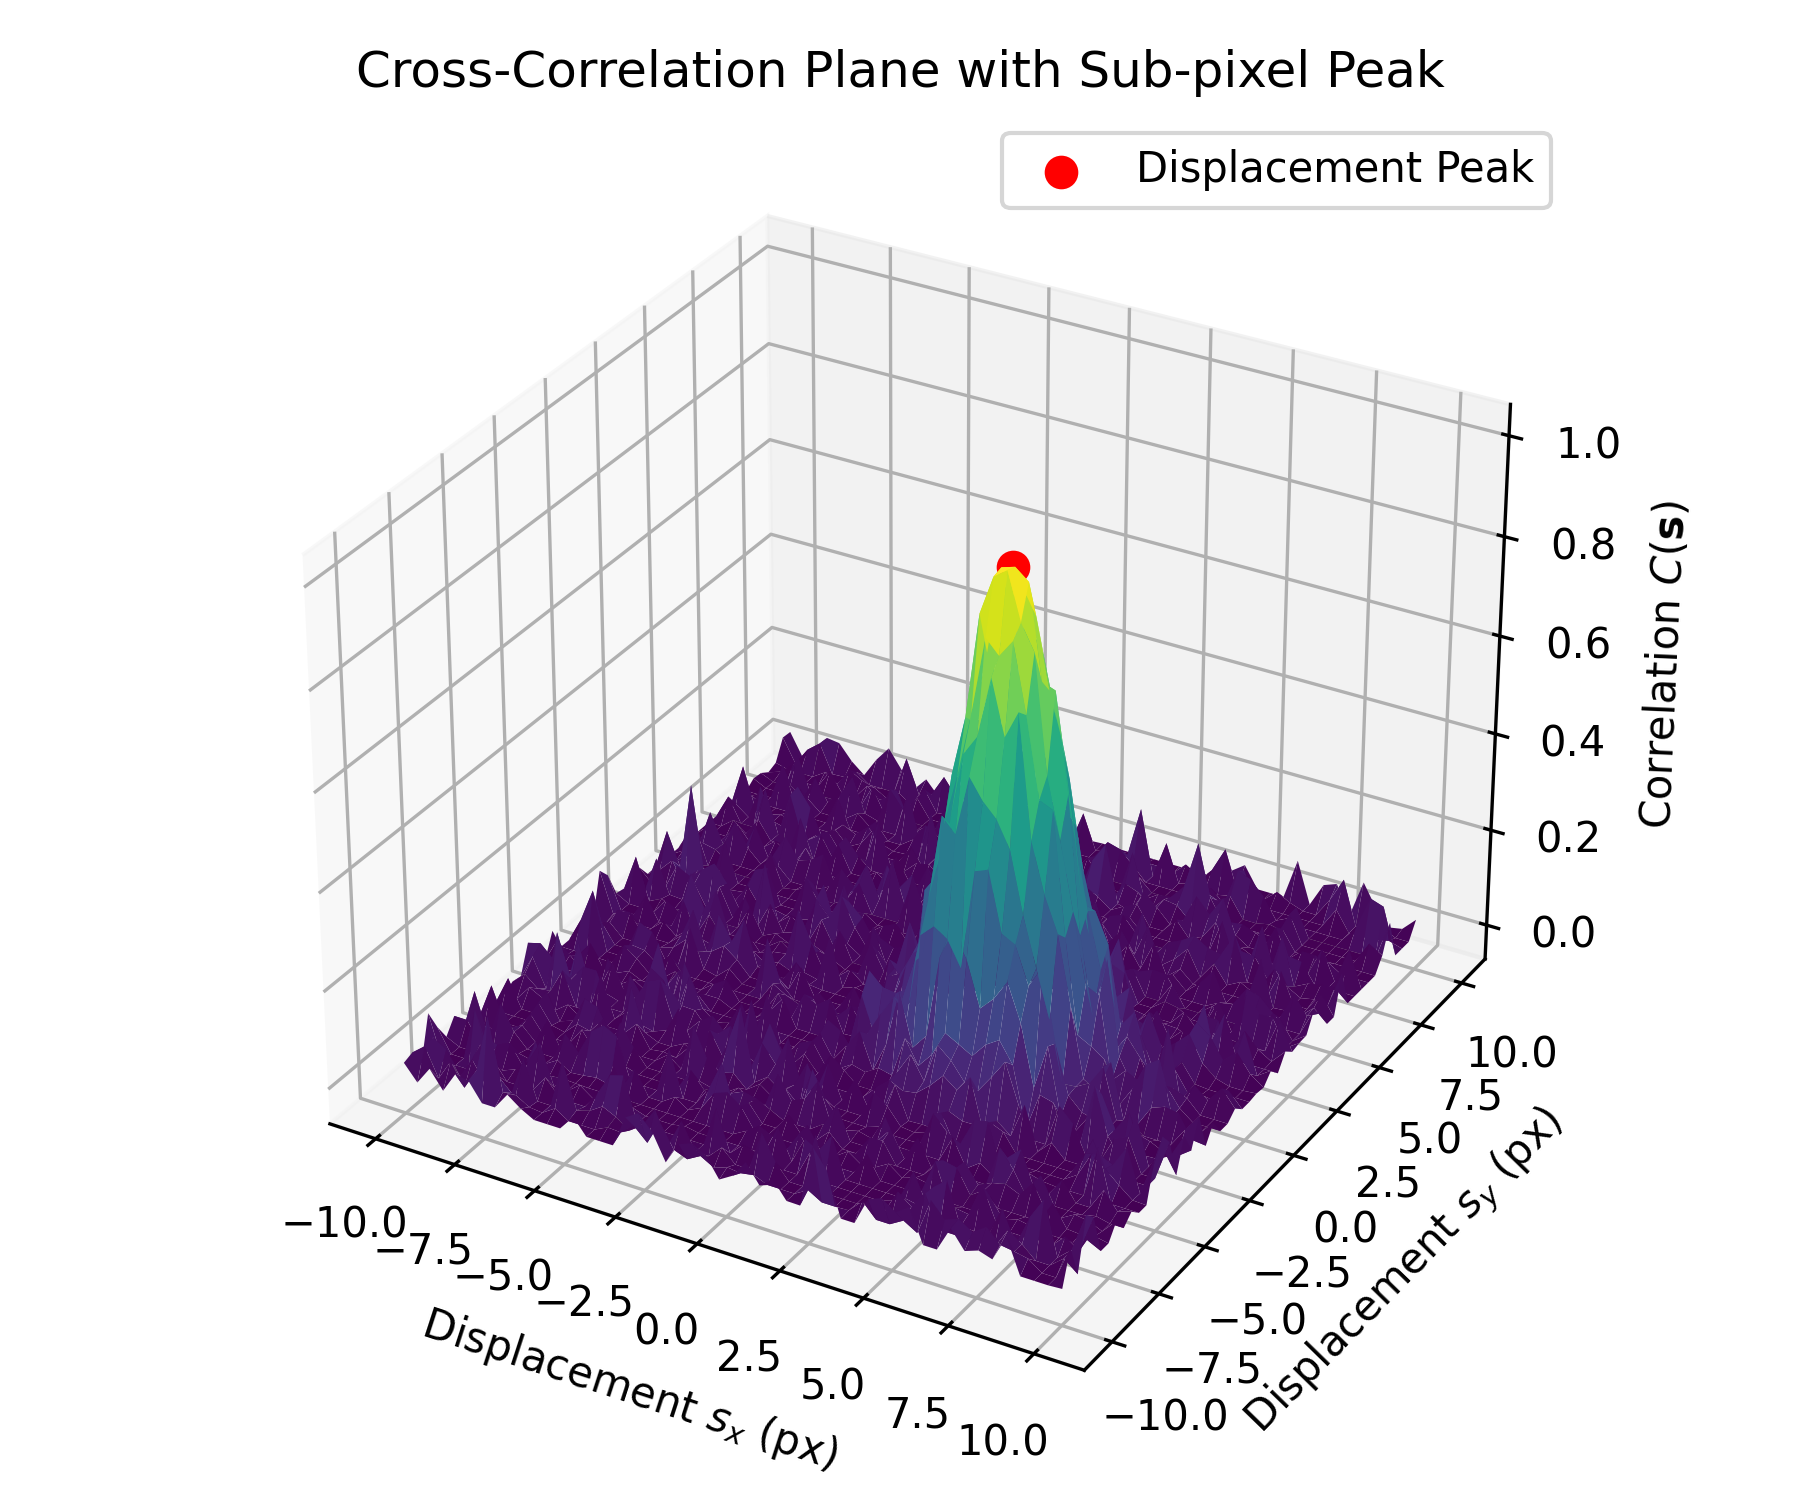
\includegraphics[width=0.9\linewidth]{correlation_peak.png}
    \end{tcolorbox}
    \caption{3D representation of the cross-correlation plane $C(\mathbf{s})$ showing the sub-pixel correlation peak that identifies the most probable displacement vector.}
    \label{fig:correlation}
\end{figure}

\vspace{0.5em}
\textbf{\color{deepblue}Step 6 -- Velocity Calculation}

Physical velocity is recovered as:
\begin{mathbox}
\begin{equation}
    \mathbf{u} = \frac{\mathbf{d} \cdot M_{\text{scale}}}{\Delta t}
\end{equation}
where $M_{\text{scale}}$ (mm/pixel) is the image magnification obtained from calibration.
\end{mathbox}

\vspace{0.5em}
\textbf{\color{deepblue}Step 7 -- Vector Validation}

Spurious vectors (outliers) are detected using:
\begin{itemize}[noitemsep, leftmargin=1.5em]
    \item[\color{accentpurple}\faIcon{check}] \textbf{Normalized Median Test (NMT):} A vector is flagged if it deviates from the median of its neighbors by more than a threshold.
    \item[\color{accentpurple}\faIcon{check}] \textbf{Signal-to-Noise Ratio (SNR):} Ratio of primary to secondary correlation peak.
\end{itemize}
Outliers are replaced by interpolation from neighboring valid vectors.
\end{answerbox}

% --------------------------------------------------------------
\subsection{Q5: What is a PIV software?}
% --------------------------------------------------------------

\begin{questionbox}
What is a PIV software? Are there well-known examples?
\end{questionbox}

\begin{answerbox}
A \textbf{\color{accentblue}PIV software} is a program that automates the complete processing pipeline: reading raw image pairs, running cross-correlation algorithms, validating vectors, and visualizing the resulting velocity field.

\vspace{0.5em}
\begin{center}
\renewcommand{\arraystretch}{1.4}
\begin{tabularx}{\linewidth}{>{\bfseries\color{deepblue}}l l X}
\toprule
\tablemark Software & \tablemark Type & \tablemark Notes \\
\midrule
\rowcolor{tablegray}
DaVis (LaVision) & Commercial & Industry standard, very feature-rich \\
PIVlab & Free / MATLAB & Most widely used in academia, open-source \\
\rowcolor{tablegray}
OpenPIV & Free / Python & Open-source, Python + GPU support \\
INSIGHT 4G (TSI) & Commercial & Used with TSI hardware systems \\
\rowcolor{tablegray}
fluidimage / mpivpy & Free / Python & Research-oriented, Python ecosystem \\
\bottomrule
\end{tabularx}
\end{center}

\vspace{0.3em}
\textbf{PIVlab} is especially popular because it is open-source, runs in MATLAB, and implements state-of-the-art algorithms with a graphical user interface.
\end{answerbox}

% --------------------------------------------------------------
\subsection{Q6: What are the most important modules for a PIV software?}
% --------------------------------------------------------------

\begin{questionbox}
What are the most important modules that a PIV software must have?
\end{questionbox}

\begin{answerbox}

\textbf{\color{deepblue}\faIcon{image}~1. Image Pre-processing Module}

Improves image quality before correlation: background subtraction, intensity normalization, CLAHE (Contrast Limited Adaptive Histogram Equalization), and masking of solid walls.

\vspace{0.5em}
\textbf{\color{deepblue}\faIcon{cogs}~2. Interrogation / Cross-Correlation Engine}

The core computational module: FFT-based cross-correlation, multi-pass iterative window refinement, and ensemble correlation for low-seeding-density flows.

\vspace{0.5em}
\textbf{\color{deepblue}\faIcon{filter}~3. Vector Validation Module}

Detects and replaces outliers using the Normalized Median Test, global SNR filtering, and iterative interpolation.

\vspace{0.5em}
\textbf{\color{deepblue}\faIcon{chart-area}~4. Post-processing Module}

Derives secondary quantities from the velocity field:
\begin{mathbox}
\begin{equation}
    \omega_z = \frac{\partial v}{\partial x} - \frac{\partial u}{\partial y} \quad \text{(vorticity)}
\end{equation}
Also: divergence, strain rate, turbulent kinetic energy, Reynolds stresses.
\end{mathbox}

\vspace{0.5em}
\textbf{\color{deepblue}\faIcon{ruler}~5. Calibration Module}

Converts pixel displacements to physical units using a reference calibration target (dot grid or checkerboard). Also corrects lens distortion.

\vspace{0.5em}
\textbf{\color{deepblue}\faIcon{palette}~6. Visualization Module}

Vector field plots, color-contoured scalar maps, streamline plots, and time-series animations.

\vspace{0.5em}
\textbf{\color{deepblue}\faIcon{file-export}~7. I/O Module}

Reads raw camera images (TIFF, BMP, HDF5) and exports results (ASCII, HDF5, VTK) for further CFD post-processing.
\end{answerbox}

% --------------------------------------------------------------
\subsection{Q7: What are the mathematical techniques used in PIV software?}
% --------------------------------------------------------------

\begin{questionbox}
What are the specific mathematical techniques implemented inside PIV software?
\end{questionbox}

\begin{answerbox}

\textbf{\color{accentpurple}\faIcon{vector-square}~1. Window Deformation (Image Deformation PIV)}

The interrogation window in $I_2$ is \textbf{deformed} according to the local velocity gradient using bilinear or B-spline interpolation:
\begin{mathbox}
\begin{equation}
    I_2^{\text{def}}(\mathbf{x}) = I_2\!\left(\mathbf{x} + \mathbf{u}(\mathbf{x})\cdot\Delta t\right)
\end{equation}
This significantly improves accuracy near shear layers.
\end{mathbox}

\vspace{0.5em}
\textbf{\color{accentpurple}\faIcon{layer-group}~2. Multi-Resolution / Multi-Pass Algorithm}

A pyramid approach: Pass~1 uses large IW ($64\times64$, coarse), Pass~2 uses $32\times32$, Pass~3 uses $16\times16$ with the previous result as the initial offset. This reduces peak-locking artifacts.

\vspace{0.5em}
\textbf{\color{accentpurple}\faIcon{crosshairs}~3. Sub-pixel Interpolation Schemes}

Gaussian 3-point fit (most common), parabolic fit, or centroid method -- all achieve 0.05--0.1 pixel accuracy.

\vspace{0.5em}
\textbf{\color{accentpurple}\faIcon{calculator}~4. Spatial Differentiation}

Velocity gradients via central finite differences:
\begin{mathbox}
\begin{equation}
    \frac{\partial u}{\partial x} \approx \frac{u_{i+1,j} - u_{i-1,j}}{2\Delta x}
\end{equation}
\end{mathbox}

\vspace{0.5em}
\textbf{\color{accentpurple}\faIcon{wave-square}~5. Reynolds Decomposition and Turbulence Statistics}

For $N$ instantaneous fields:
\begin{mathbox}
\begin{equation}
    u(\mathbf{x}, t_n) = \bar{u}(\mathbf{x}) + u'(\mathbf{x}, t_n), \qquad
    \bar{u} = \frac{1}{N}\sum_{n=1}^{N} u(\mathbf{x}, t_n)
\end{equation}
Turbulent kinetic energy:
\begin{equation}
    k = \frac{1}{2}\!\left(\overline{u'^2} + \overline{v'^2}\right)
\end{equation}
\end{mathbox}

\vspace{0.5em}
\textbf{\color{accentpurple}\faIcon{project-diagram}~6. Proper Orthogonal Decomposition (POD)}

Applied to time-series PIV data to extract dominant flow structures ordered by energy content (snapshot method):
\begin{mathbox}
\begin{equation}
    \mathbf{u}(\mathbf{x}, t) = \sum_{i=1}^{N} a_i(t)\,\boldsymbol{\phi}_i(\mathbf{x})
\end{equation}
\end{mathbox}

\vspace{0.5em}
\textbf{\color{accentpurple}\faIcon{chart-line}~7. Spectral Analysis}

Spatial power spectral density via 2D FFT of velocity fluctuation fields; used to verify turbulent energy cascades following Kolmogorov's $-5/3$ law.

\vspace{0.5em}
\textbf{\color{accentpurple}\faIcon{brain}~8. Optical Flow and Deep Learning Methods}

Modern PIV software optionally uses optical flow algorithms (Horn--Schunck, Lucas--Kanade) or CNN-based approaches (e.g., LiteFlowNet adapted for PIV), achieving higher spatial resolution than correlation-based methods.
\end{answerbox}

% --------------------------------------------------------------
\subsection{Q8: What is the Stokes number in more detail?}
% --------------------------------------------------------------

\begin{questionbox}
You mentioned the Stokes number earlier. Can you explain it in more detail?
\end{questionbox}

\begin{answerbox}
The \textbf{\color{accentpurple}Stokes number} ($St$) quantifies how well a particle follows the fluid flow:

\begin{mathbox}
\begin{equation}
    St = \frac{\tau_p}{\tau_f}
\end{equation}
\end{mathbox}

\textbf{Particle relaxation time} for a spherical particle in the Stokes drag regime:
\begin{mathbox}
\begin{equation}
    \tau_p = \frac{\rho_p\, d_p^2}{18\,\mu_f}
\end{equation}
where $\rho_p$ is the particle density, $d_p$ is the particle diameter, and $\mu_f$ is the dynamic viscosity of the fluid.
\end{mathbox}

\vspace{0.5em}
\textbf{\color{deepblue}Interpretation:}
\begin{itemize}[noitemsep, leftmargin=1.5em]
    \item[\color{accentgreen}\faIcon{check-circle}] $St \ll 1$: Particle follows the fluid perfectly --- ideal PIV tracer.
    \item[\color{accentorange}\faIcon{exclamation-circle}] $St \approx 1$: Particle starts to deviate from the fluid streamlines.
    \item[\color{accentred}\faIcon{times-circle}] $St \gg 1$: Particle motion is dominated by inertia, independent of the flow.
\end{itemize}
In practice, PIV particles are designed to satisfy $St < 0.1$.
\end{answerbox}

% --------------------------------------------------------------
\subsection{Q9: What are the limitations of PIV?}
% --------------------------------------------------------------

\begin{questionbox}
What are the limitations and weak points of PIV as a technique?
\end{questionbox}

\begin{answerbox}

\begin{warningbox}{Limitations of PIV}
\begin{enumerate}[leftmargin=1.5em]
    \item \textbf{\color{accentred}Optical access required:} The flow domain must have transparent walls. Impossible in many industrial settings (metal pipes, engines).
    \item \textbf{\color{accentred}2D projection problem:} Standard 2D PIV measures only two velocity components. The out-of-plane component ($w$) is lost. Stereoscopic PIV (3C-2D) or Tomographic PIV (3D) address this but at higher cost.
    \item \textbf{\color{accentred}Seeding quality is critical:} Non-uniform seeding creates void regions; over-seeding causes particle overlap. Maintaining $\sim$5--10 particle pairs per IW is practically challenging.
    \item \textbf{\color{accentred}Spatial resolution limit:} Features smaller than the interrogation window are spatially filtered out.
    \item \textbf{\color{accentred}High-speed flows:} Very fast flows require sub-microsecond $\Delta t$ and high-frame-rate cameras --- expensive hardware.
    \item \textbf{\color{accentred}Near-wall measurements:} Laser reflection from solid walls creates a glare region that obscures particle images near the wall ($y^+ < 5$), making accurate boundary layer measurement difficult.
    \item \textbf{\color{accentred}Temporal resolution:} Standard double-frame PIV yields one velocity field per laser shot pair. Time-resolved PIV (TR-PIV) requires high-repetition-rate lasers and high-speed cameras.
\end{enumerate}
\end{warningbox}

\end{answerbox}

% --------------------------------------------------------------
\subsection{Q10: Raw Follow-up on Near-Wall Limitations}
% --------------------------------------------------------------

\textbf{Student (Raw Prompt):} "You said laser reflection makes near-wall measurements hard. Is there any trick to fix that or are we just blind near the wall?"

\bigskip
\textbf{LLM Answer:}

We are not entirely blind, but it requires special tricks! The most common workarounds are:
\begin{itemize}[noitemsep]
    \item \textbf{Fluorescent particles:} Using Rhodamine-B dyed particles and placing an optical filter in front of the camera. The filter blocks the glaring green laser light (532 nm) but lets the orange fluorescent emitted light (around 580 nm) pass through.
    \item \textbf{Painting the wall:} Coating the background/wall with black matte paint (or Rhodamine paint) to absorb the laser sheet and reduce reflections.
    \item \textbf{Index matching:} Matching the refractive index of the fluid with the solid wall material if possible.
\end{itemize}

% ==============================================================
\section{Summary of Lessons Learned}
% ==============================================================

\begin{summarybox}{Key Takeaways}
\begin{itemize}[leftmargin=1.5em]
    \item[\color{accentgreen}\faIcon{check}] PIV is a non-intrusive whole-field optical velocimetry technique based on tracking particle displacements between two laser-illuminated frames.
    \item[\color{accentgreen}\faIcon{check}] The core mathematics relies on FFT-accelerated cross-correlation of particle image pairs, with sub-pixel Gaussian peak fitting for accuracy.
    \item[\color{accentgreen}\faIcon{check}] The Stokes number ($St \ll 1$) is the fundamental criterion for choosing tracer particles that faithfully follow the flow.
    \item[\color{accentgreen}\faIcon{check}] Key hardware components are a double-pulsed Nd:YAG laser, a CCD/sCMOS double-frame camera, a hardware synchronizer, and seeding particles.
    \item[\color{accentgreen}\faIcon{check}] Advanced software modules implement window deformation, multi-pass iterative refinement, POD decomposition, and even deep learning-based optical flow.
    \item[\color{accentgreen}\faIcon{check}] 2D PIV only measures two out of three velocity components --- a fundamental physical limitation addressed by stereoscopic and tomographic variants.
    \item[\color{accentgreen}\faIcon{check}] Near-wall measurements and optical access requirements are the most practically limiting constraints of PIV.
\end{itemize}
\end{summarybox}

\paragraph{Personal Reflection}
I tried running PIVlab on a sample dataset (flow past a cylinder) during this homework to see these concepts in action. I noticed that near the boundaries of the cylinder, the velocity vectors were often erroneous or chaotic unless I specifically drew a mask over the solid body. It perfectly demonstrated the "near-wall measurements" limitation discussed with the LLM. Furthermore, tweaking the interrogation window size down to $16 \times 16$ drastically improved the resolution of the small turbulent eddies in the wake, though it increased the processing time significantly.

% ==============================================================
\section{Discussion on Weak Points of the LLM}
% ==============================================================

\begin{warningbox}{Critical Observations}
\begin{enumerate}[leftmargin=1.5em]
    \item \textbf{\color{accentorange}Omission of Shake-The-Box (STB):} The LLM did not spontaneously mention \textit{Shake-The-Box}, a state-of-the-art Lagrangian particle tracking method that outperforms classical tomographic PIV in 3D flows. This is a significant modern development that a complete answer should have included.
    \item \textbf{\color{accentorange}Deep learning claims:} The LLM cited LiteFlowNet adapted for PIV as a deep learning technique. While conceptually correct, the specific network name should be verified against the latest literature (e.g., PIV-LiteFlowNet-en by Cai et al., 2019), as the field evolves rapidly. The LLM did not provide bibliographic references.
    \item \textbf{\color{accentorange}No mention of Micro-PIV:} Micro-PIV for microscale biological flows was only briefly mentioned in passing (Q1 table) but not discussed as a distinct variant with its own challenges (evanescent wave illumination, Brownian motion noise, depth-of-field effects).
    \item \textbf{\color{accentorange}Ensemble correlation not elaborated:} The LLM listed ensemble correlation as a module feature but did not explain it in detail. Ensemble/sum-of-correlation is a critical technique for low-seeding-density flows and deserved more explanation.
    \item \textbf{\color{accentorange}No uncertainty quantification discussion:} Modern PIV software includes uncertainty quantification (UQ) methods (e.g., peak-ratio methods, correlation statistics). The LLM did not mention this aspect at all.
\end{enumerate}
\end{warningbox}

\vspace{0.5em}
\begin{tcolorbox}[
    enhanced,
    colback=lightblue!15!white,
    colframe=accentblue!50!white,
    boxrule=0.5pt,
    arc=3pt,
    left=10pt, right=10pt, top=8pt, bottom=8pt
]
\faIcon{book}\;\textit{These gaps do not indicate incorrect answers but rather incomplete coverage. The student verified the provided information against Raffel et al.\ \textbf{Particle Image Velocimetry: A Practical Guide} (3rd ed., Springer, 2018) and found the core content to be accurate.}
\end{tcolorbox}

\end{document}
